\documentclass[12,french]{report}
\usepackage{geometry}
\geometry{vmargin=3cm, hmargin=3cm}
\usepackage[T1]{fontenc}
\usepackage[utf8]{inputenc}
\usepackage[french]{babel}
\usepackage{graphicx}
\usepackage{amsmath}
\usepackage{amssymb}
\usepackage{sectsty}
\usepackage{authblk}
\usepackage{algpseudocode}
\usepackage{algorithm}
\usepackage{xspace}
\usepackage{mathtools}
\usepackage{mathrsfs}
\usepackage{enumitem}
\usepackage{titlesec}
\usepackage{hyperref}
\usepackage{xcolor}
\usepackage{caption}
\usepackage{float}
\usepackage{tabto}


%\AddThinSpaceBeforeFootnotes
%\FrenchFootnotes

\titleformat{\chapter}[hang]{\bf\Huge}{\thechapter.}{2pc}{}
\titlespacing*{\chapter}{10pt}{0pt}{40pt}[0pt]
\newcommand{\HRule}{\rule{\linewidth}{0.5mm}}

\providecommand{\keywords}[1]{\textbf{\textit{Keywords:}} #1}
\bibliographystyle{apalike}

\usepackage{hyperref}

\begin{document}
\hypersetup{pdfborder=0 0 0}

\begin{titlepage}

\begin{center}
	\vspace*{\stretch{1}}
	\textsc{{\LARGE Institut national des sciences appliquées de Rouen} \\ 			\vspace{6mm} {\Large INSA de Rouen}} \\
	\vspace{5mm}
	
\includegraphics[width=0.4\textwidth]{./Images/insa}\\[1.0 cm]

	\textsc{\Large Projet Info GM3 - Vague 1 - Sujet 2}\\[0.5cm]

	% Title
	\HRule \\[0.5cm]
	{ \Huge \bfseries Jeu de la vie}\\[0.2cm]
	\HRule \\[0.95cm]

\begin{figure}[H]
    \begin{minipage}[c]{.46\linewidth}
        \centering
        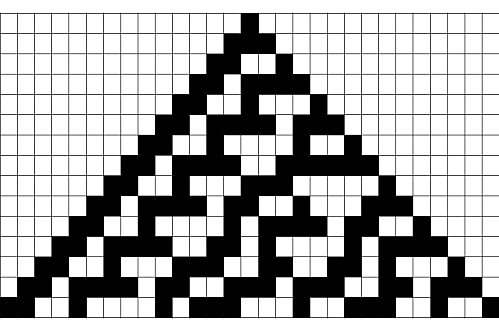
\includegraphics[width=0.8\textwidth]{./Images/2}\\[0.9 cm]
    \end{minipage}
    \hfill%
    \begin{minipage}[c]{.46\linewidth}
        \centering
        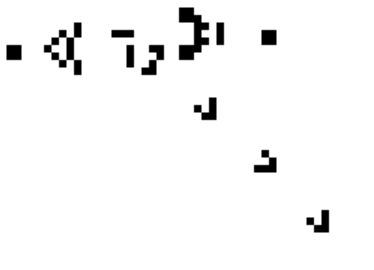
\includegraphics[width=0.8\textwidth]{./Images/1}\\[0.9 cm]
    \end{minipage}
\end{figure}\vspace{0.6cm}

	% Author and supervisor
	\begin{minipage}{0.4\textwidth}
		\begin{flushleft} \large
			\emph{Auteurs:}\\
			Thibaut \textsc{André-Gallis} \\
			{\small\href{mailto:thibaut.andregallis@insa-rouen.fr}{thibaut.andregallis@insa-rouen.fr}} \\
			Kévin \textsc{Gatel} \\
			{\small\href{mailto:kevin.gatel@insa-rouen.fr}{kevin.gatel@insa-				rouen.fr}}
		\end{flushleft}
	\end{minipage}
	\begin{minipage}{0.4\textwidth}
		\begin{flushright} \large
			\emph{Enseignant:} \\
			Julien \textsc{Saunier} \\
			{\small\href{mailto:julien.saunier@insa-rouen.fr}								{julien.saunier@insa-rouen.fr}}
		\end{flushright}
	\end{minipage}
	\vspace*{\stretch{1}}

	\vfill
	{\large 16 Octobre 2020}
\end{center}
\end{titlepage}

\tableofcontents

\listoffigures

\renewcommand{\chaptername}{}
\chapter*{Introduction}
%\label{chapter:Introduction}
\addcontentsline{toc}{chapter}{Introduction}

Le jeu de la vie est un programme informatique imaginé par John Conway dans les années 70. Ce dernier est un mathématicien britannique née en 1937. Il vient de décéder il y a un mois à cause du Coronavirus. Ses travaux tournent autour des théories de groupes ainsi que les jeux combinatoires.

Depuis presque 50 ans ce jeu fascine les mathématiciens, les informaticiens mais aussi les biologistes et les philosophes. En effet il nous montre comment un système évoluant selon des règles simplistes peut engendrer des résultats incroyablement riches.\\

Il faut préciser que le jeu de la vie n'est pas vraiment un jeu au sens ludique, puisqu'il ne nécessite aucun joueur. Il s'agit simplement d'entrée une configuration initiale et de regarder son évolution. 

C'est l'analogie entre ces règles et certains critères d'évolution de populations de bactéries qui a conduit à donner à cet automate le nom de jeu de la vie.\\

Dans ce projet, nous allons étudier le jeu de la vie à travers son implémentation en C\footnote{Le \textit{main.c} est le programme principal, la grille initiale est définie dans les fichiers \textit{fgrille}}. Nous allons décrire le programme, montrer sa modélisation à partir de plusieurs dispositions initiales et fournir quelques analyses sur les résultats du jeu.

\chapter{Principe du jeu}

Le jeu se déroule sur une grille à deux dimensions, théoriquement infinie (dans la pratique sa taille sera finie), dont les cases qu'on appelle des cellules (par analogie avec les cellules vivantes) peuvent prendre deux états distincts : vivantes ou mortes. On peut ainsi voir ce petit programme comme un automate cellulaire.\\

 Le fonctionnement est très simple. L'état de l'automate à l'étape $n$ est uniquement fonction de son état à l'étape $n-1$. L'évolution de l'état d'une cellule dépend de l'état de ses 8 cellules voisines.\\

Dans l'automate de Conway, les règles sont les suivantes :
\begin{itemize}[label=\textbullet]
	\item Une cellule morte à l'étape $n-1$ et ayant exactement 3 cellules voisines vivantes deviendra vivante à l'étape suivante. (naissance liée à un environnement optimal)
	\item Une cellule vivante à l'étape $n-1$ et ayant 2 ou 3 cellules voisines vivantes sera maintenue vivante à l'étape $n$ sinon elle meurt. (destruction par désertification ou surpopulation)
\end{itemize}\vspace{0.3cm}

Par exemple sur un cas très simple on aura : \vspace{0.1cm}

\begin{figure}[H]
    \begin{minipage}[c]{.46\linewidth}
        \centering
        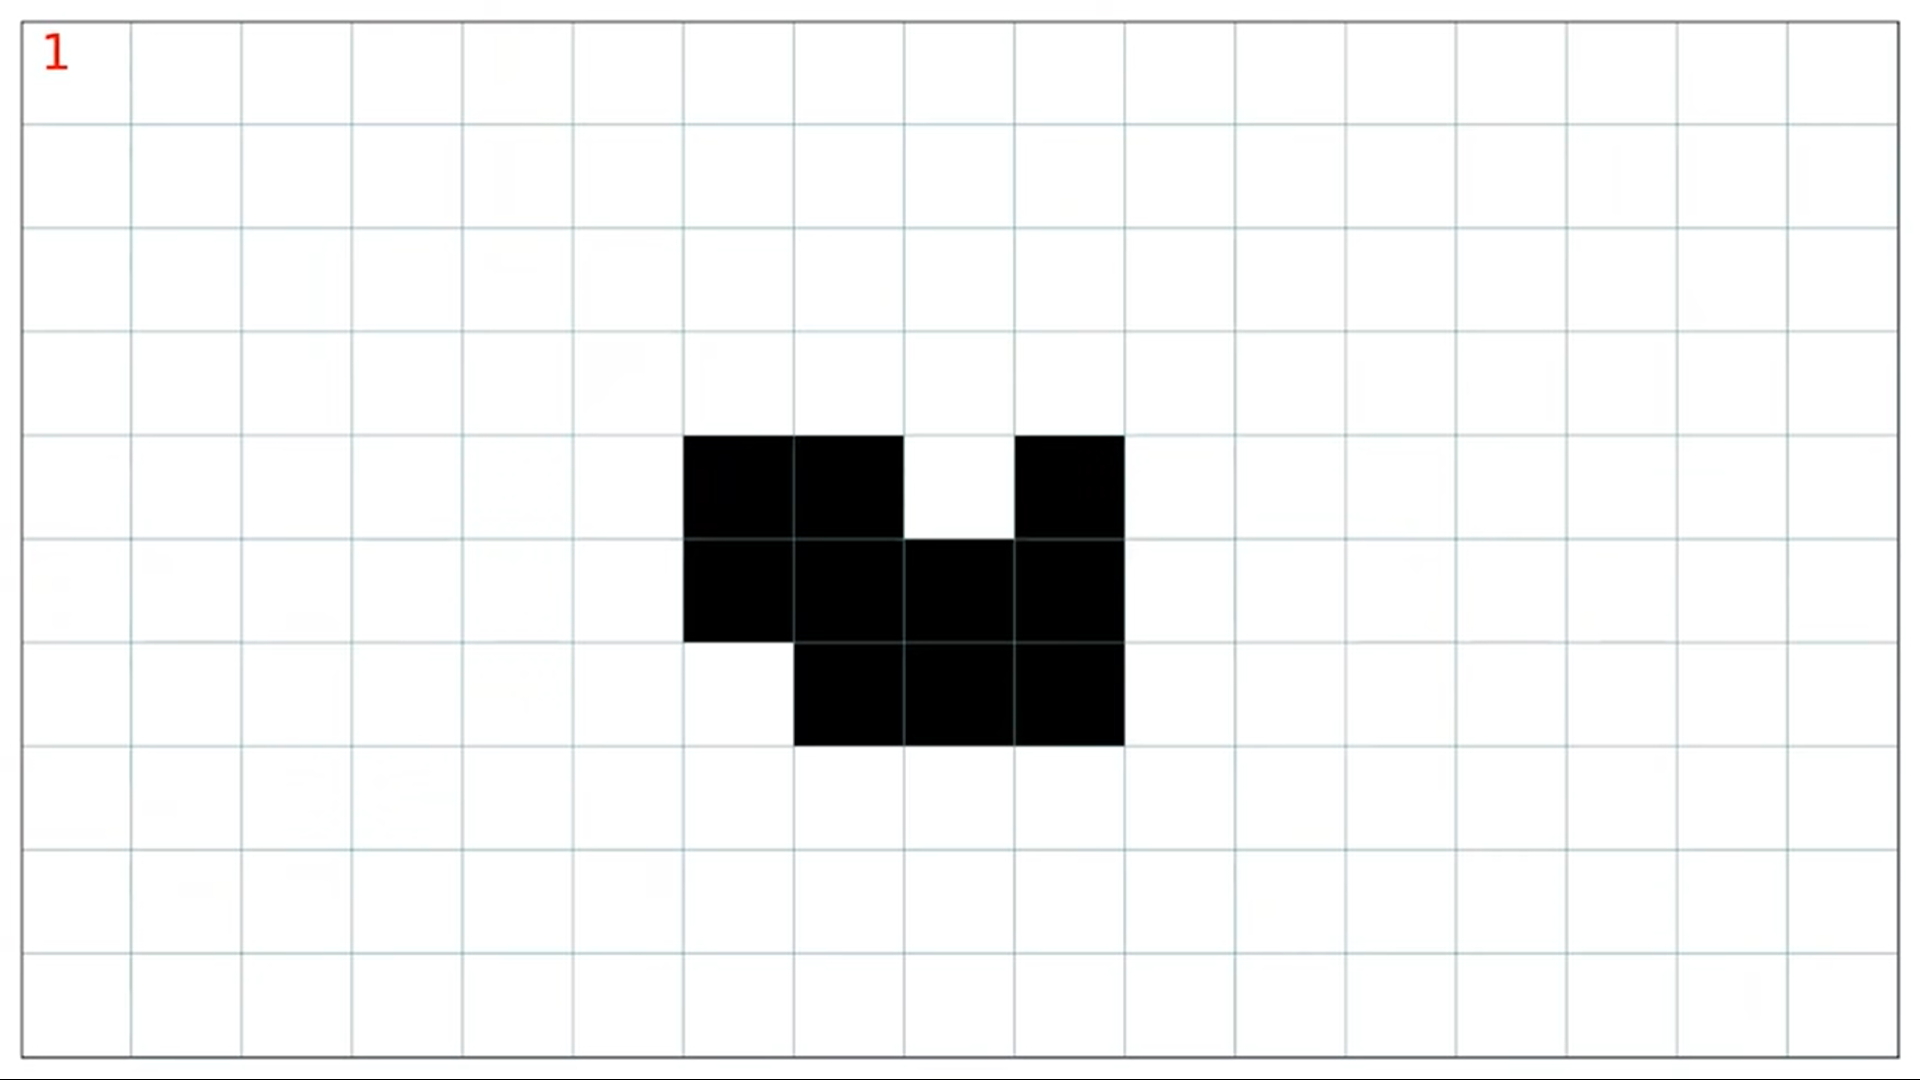
\includegraphics[width=0.9\textwidth]{./Images/3}\\
        \caption{Etape $n_{0}$}
    \end{minipage}
    \hfill%
    \begin{minipage}[c]{.46\linewidth}
        \centering
        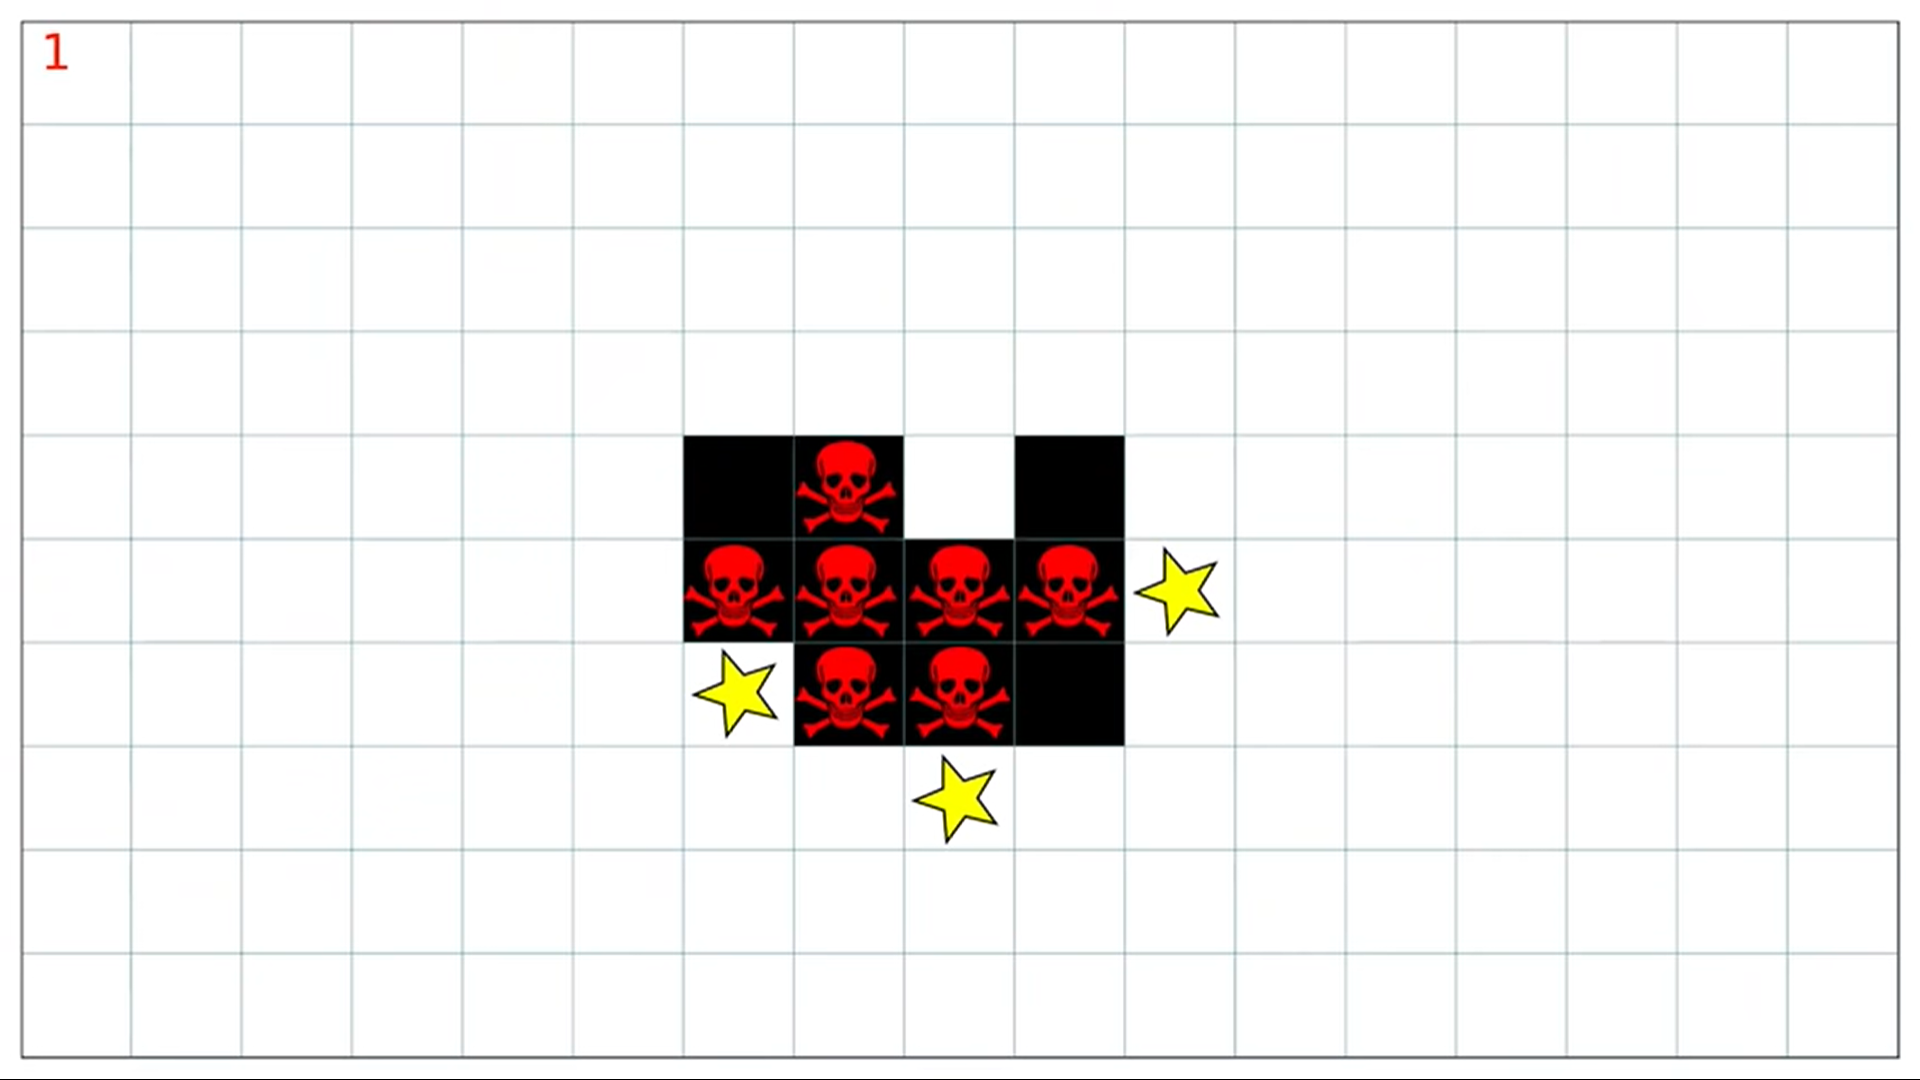
\includegraphics[width=0.9\textwidth]{./Images/4}\\
        \caption{Construction de l'étape $n_{0}+1$}
    \end{minipage}
\end{figure}%\vspace{0.1cm}

\begin{figure}[H]
	\center
	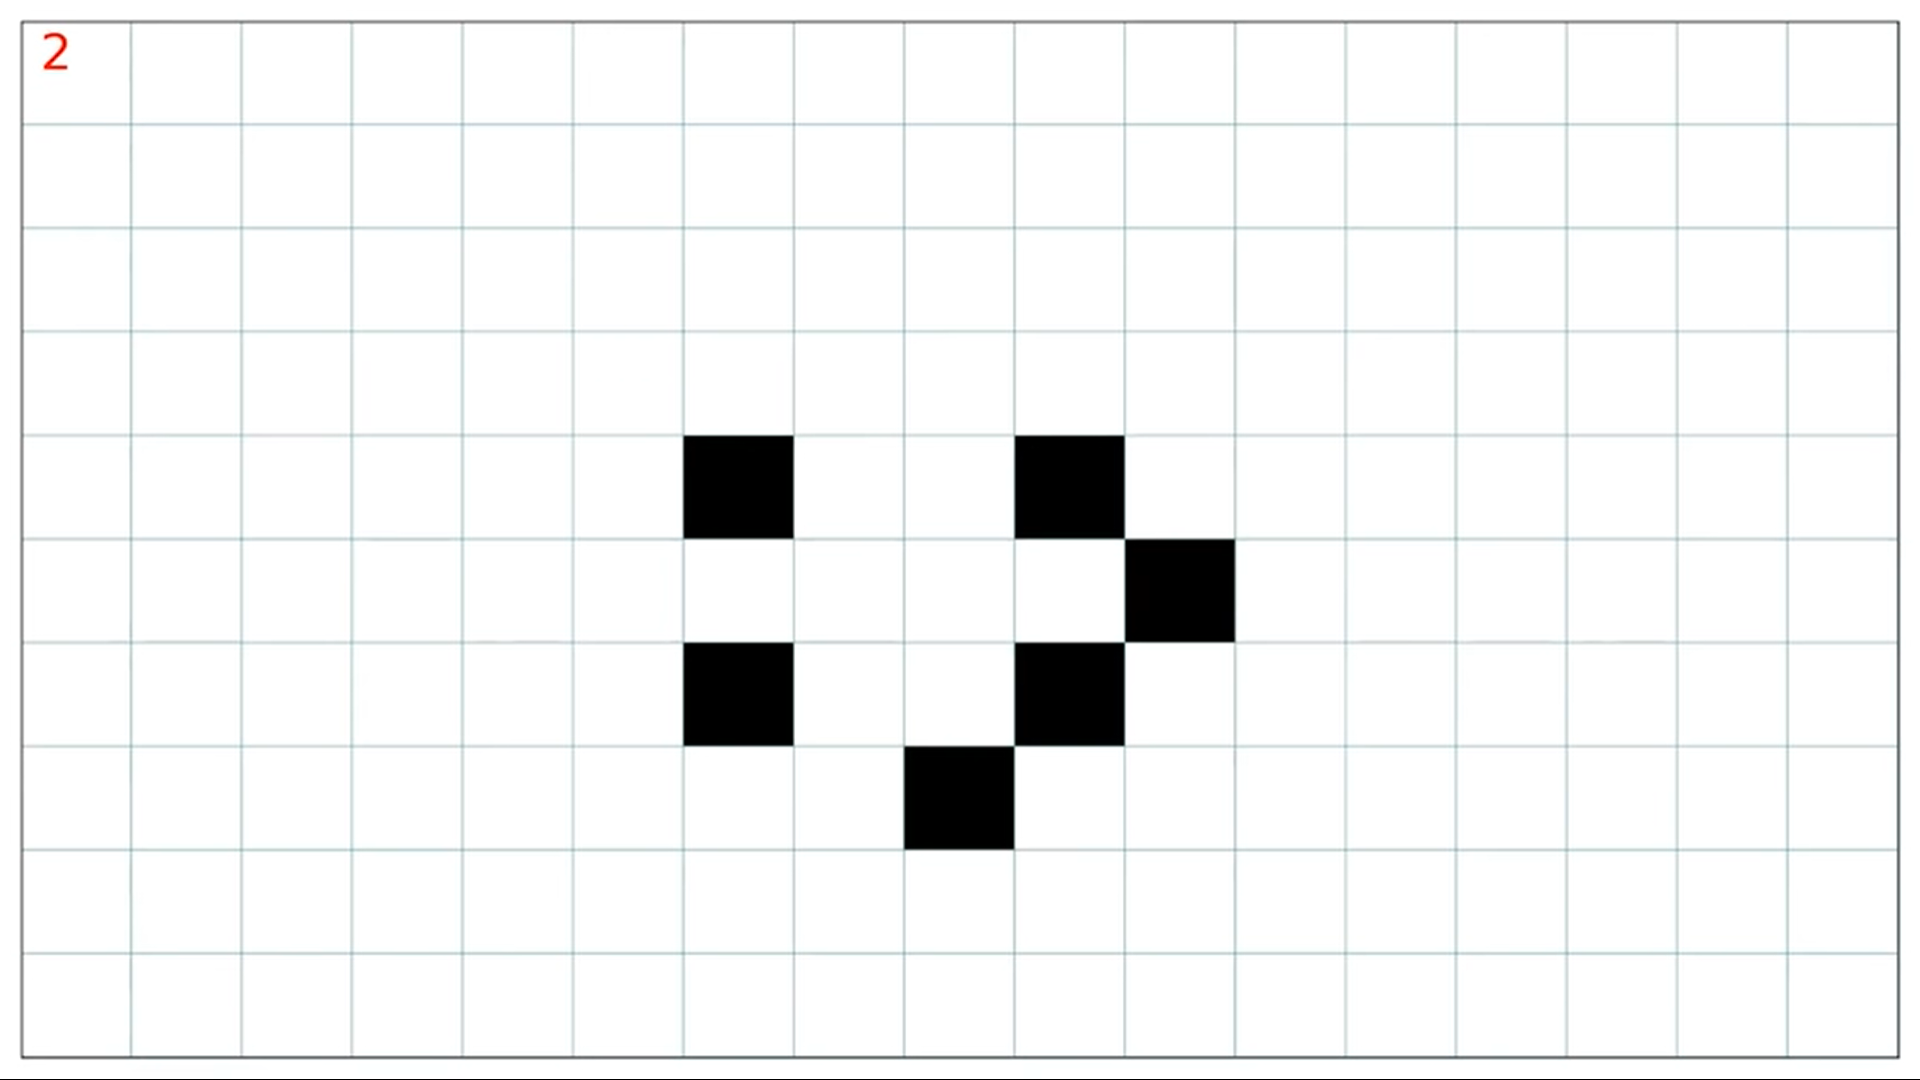
\includegraphics[width=0.45\textwidth]{./Images/5}
	\caption{Etape $n_{0}+1$}
\end{figure}\vspace{0.2cm}

Ainsi, ce processus peut être répéter autant de fois que le souhaite l'utilisateur. \\

\chapter{Généralités}

Après plusieurs parties avec des configurations initiales différentes, on retrouve plusieurs situations et on s'aperçoit que certains motifs reviennent régulièrement.\\

On observe plusieurs cas récurrents : 

\begin{itemize}[label=\textbullet]
	\item Soit les cellules finissent par mourir (ce cas n'est pas très intéressant)
	\item Soit les cellules convergent vers une ou plusieurs structures stables, ou cycliques (qui reviennent sur leur pas)
	\item Soit les cellules ont une disposition telle qu'elles progressent dans l'espace sans modifier leur structure
\end{itemize}\vspace{0.25cm}

Lorsqu'on simule avec un état initial aléatoire, nous observons ces structures sous plusieurs formes différentes.

\section{Structures Stables}

On appelle figure stable un regroupement de cellules telle qu'à l'étape $n_{0}+1$ ce regroupement soit le même que l'étape $n_{0}$. Il existe plusieurs structures stables. Parmi elles, les plus récurrentes sont \footnote{Ces quatre cas de figure peuvent être observés en mettant le fichier \textit{fgrille0} en état initial} \vspace{0.3cm} :

\begin{figure}[H]
    \begin{minipage}[c]{.46\linewidth}
        \centering
        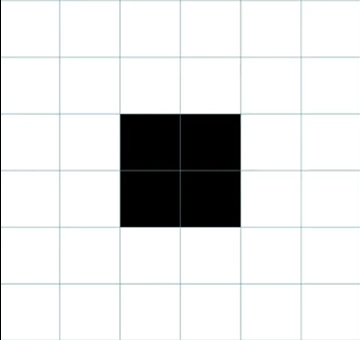
\includegraphics[width=0.55\textwidth]{./Images/6}\\
        \caption{Le bloc}
    \end{minipage}
    \hfill%
    \begin{minipage}[c]{.46\linewidth}
        \centering
        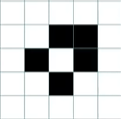
\includegraphics[width=0.55\textwidth]{./Images/7}\\
        \caption{Le bateau}
    \end{minipage}
\end{figure}%\vspace{0.1cm}

\begin{figure}[H]
    \begin{minipage}[c]{.46\linewidth}
        \centering
        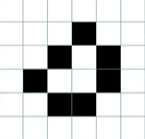
\includegraphics[width=0.55\textwidth]{./Images/8}\\
        \caption{Le pain}
    \end{minipage}
    \hfill%
    \begin{minipage}[c]{.46\linewidth}
        \centering
        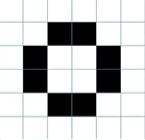
\includegraphics[width=0.55\textwidth]{./Images/9}\\
        \caption{La mare}
    \end{minipage}
\end{figure}\vspace{0.1cm}



\section{Structures cycliques}

On appelle structure cyclique ou oscillante un regroupement de cellules qui, au bout de $n$ générations, retombe sur la même structure. On dira qu'elle est de période n. Il existe également plusieurs structures cycliques ou oscillantes. On observe les plus fréquentes ci-dessous\footnote{Ces trois cas de figure peuvent être observés en mettant le fichier \textit{fgrille1} en état initial} : \vspace{0.3cm}

\begin{figure}[H]
    \begin{minipage}[c]{.46\linewidth}
        \centering
        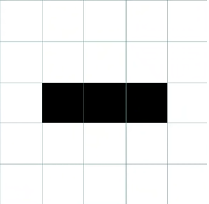
\includegraphics[width=0.6\textwidth]{./Images/10}\\
        \caption{Le clignotant $n_{0}$}
    \end{minipage}
    \hfill%
    \begin{minipage}[c]{.46\linewidth}
        \centering
        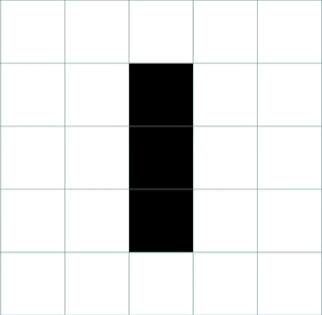
\includegraphics[width=0.6\textwidth]{./Images/10'}\\
        \caption{Le clignotant $n_{0}+1$}
    \end{minipage}
\end{figure}\vspace{0.25cm}

\begin{figure}[H]
    \begin{minipage}[c]{.46\linewidth}
        \centering
        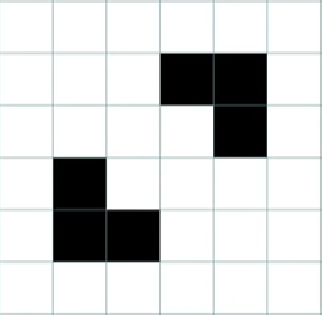
\includegraphics[width=0.6\textwidth]{./Images/11}\\
        \caption{La balise $n_{0}$}
    \end{minipage}
    \hfill%
    \begin{minipage}[c]{.46\linewidth}
        \centering
        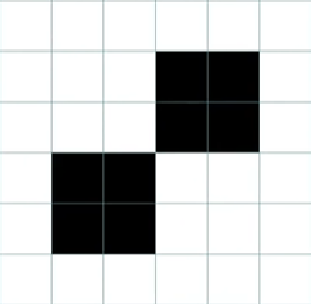
\includegraphics[width=0.6\textwidth]{./Images/11'}\\
        \caption{La balise $n_{0}+1$}
    \end{minipage}
\end{figure}\vspace{0.25cm}

\begin{figure}[H]
    \begin{minipage}[c]{.46\linewidth}
        \centering
        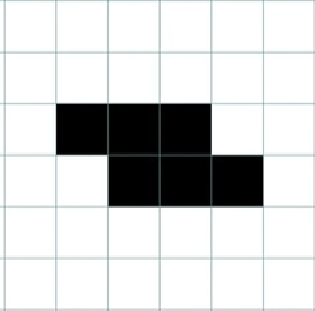
\includegraphics[width=0.6\textwidth]{./Images/12}\\
        \caption{Le crapeau $n_{0}$}
    \end{minipage}
    \hfill%
    \begin{minipage}[c]{.46\linewidth}
        \centering
        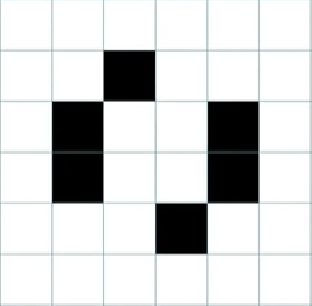
\includegraphics[width=0.6\textwidth]{./Images/12'}\\
        \caption{Le crapeau $n_{0}+1$}
    \end{minipage}
\end{figure}\vspace{0.25cm}

\pagebreak

Celles-ci sont toutes de périodes 2. Mais il en existe plein d'autres de périodes plus élevées. Par exemple celle-ci se répétera toutes les 15 générations\footnote{Ce cas de figure peut être observé en mettant le fichier \textit{fgrille2} en état initial} :  \vspace{0.3cm}

\begin{figure}[H]
	\center
	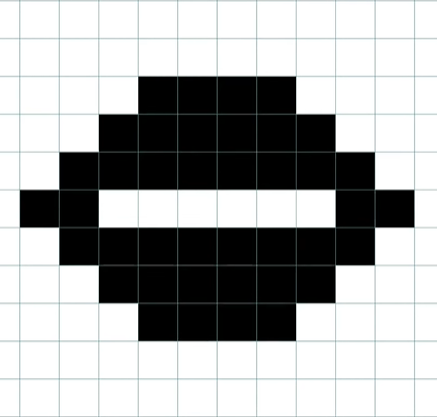
\includegraphics[width=0.5\textwidth]{./Images/13}
	\caption{Oscillateur de période 15}
\end{figure}\vspace{0.1cm}

\section{Planeurs}

Un planeur est une structure qui retrouve sa configuration en s'étant déplacé d'une case voisine. Il existe des planeurs pouvant se déplacer par la droite (engendrant les planeurs se dirigeant la gauche, par le haut et par le bas à une rotation près) comme l'exemple ci-dessous\footnote{Cette structure peut être observée en mettant le fichier \textit{fgrille3} en état initial} : \vspace{0.3cm}

\begin{figure}[H]
	\center
	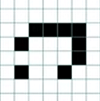
\includegraphics[width=0.3\textwidth]{./Images/14}
	\caption{Planeur de période 4}
\end{figure}\vspace{0.5cm}

Et d'autres qui peuvent se déplacer en diagonale\footnote{Cette structure peut être observée en mettant le fichier \textit{fgrille4} en état initial} : \vspace{0.3cm}

\begin{figure}[H]
	\center
	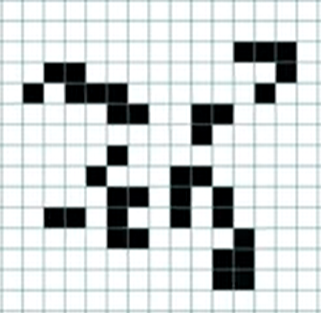
\includegraphics[width=0.4\textwidth]{./Images/15}
	\caption{L'oie du canada}
\end{figure}\vspace{0.1cm}

\section{Canons à planeurs}

Les canons à planeurs sont les structures qui, lorsqu'elles retrouvent leur configuration initiale, émettent un ou plusieurs planeurs. \footnote{Le canon peut être observé en mettant le fichier \textit{fgrille5} en état initial} : \vspace{0.3cm}

\begin{figure}[H]
	\center
	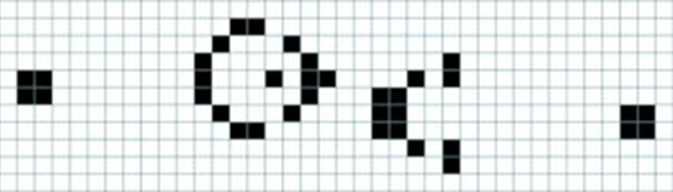
\includegraphics[width=0.9\textwidth]{./Images/16}
	\caption{Canon à planeurs de Gosper}
\end{figure}\vspace{0.1cm}

La découverte d'une telle structure a provoqué une révolution dans le jeu de la vie. Celle-ci nous montre qu'avec un nombre fini de cellule, il est possible d'en créer avec intervalle régulier, soit une infinité.

\chapter{Programme}
\section{Indications d'utilisation}

La taille d’un tableau doit être définie comme constante lors de la compilation d’un programme.
Pour optimiser cette espace, nous avons décidé de la mettre en paramètre dans le programme qu’on
décide arbitrairement selon la taille souhaitée.\\

Ainsi, il est important lors de la compilation du programme, de définir la variable N au niveau du
\#define dans le main.c puisqu’elle définit la taille du tableau à deux dimensions contenant toutes les
cellules.\\

On aura alors pour l’appel des fichiers fgrille0, fgrille1, fgrille2 et fgrille3, un N devant être égale
à 22. Pour les fichiers fgrille4 et fgrille5, N devra être égale à 45. Pour ce cas de figure, n’oubliez pas
d’ouvrir le terminal en grand pour un meilleur affichage.

\section{Pseudo-code}

\begin{center}

	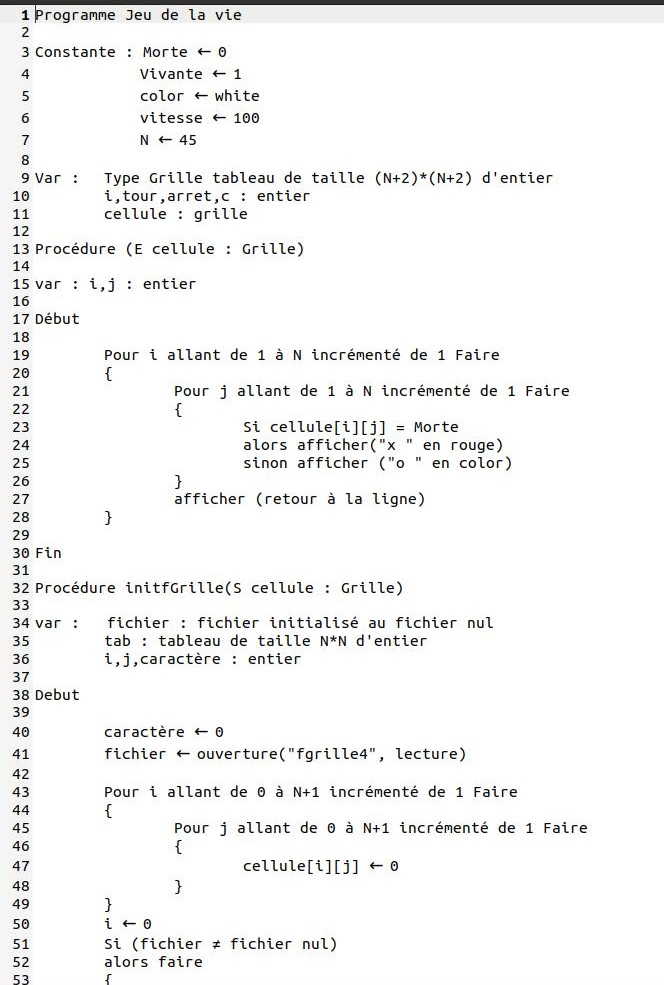
\includegraphics[width=0.8\textwidth]{./Images/Pseudo_code_1'}\\
	
	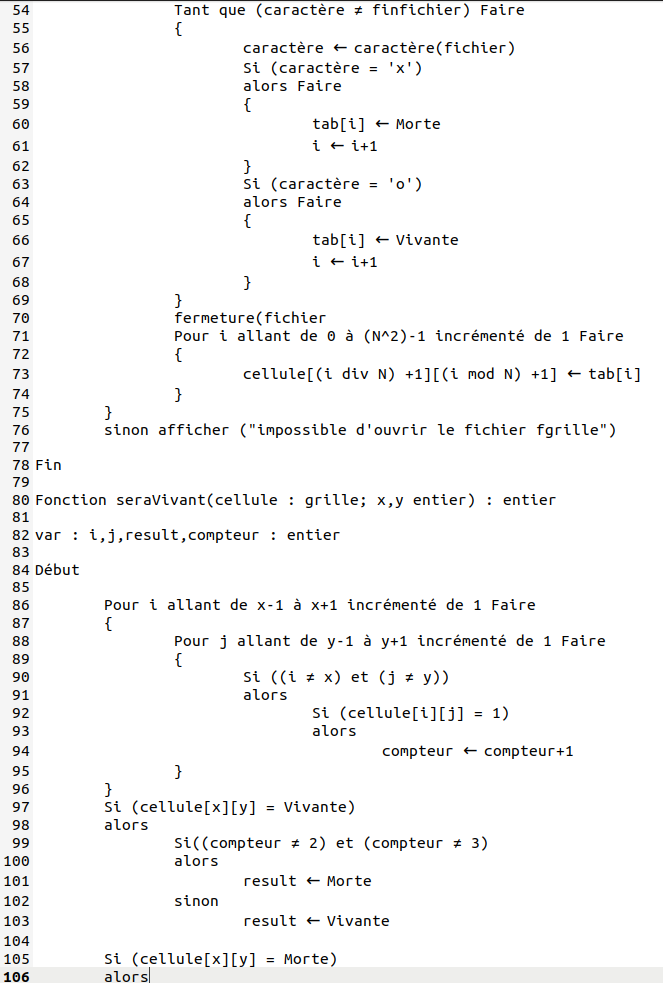
\includegraphics[width=0.95\textwidth]{./Images/Pseudo_code_2'}\\
	
	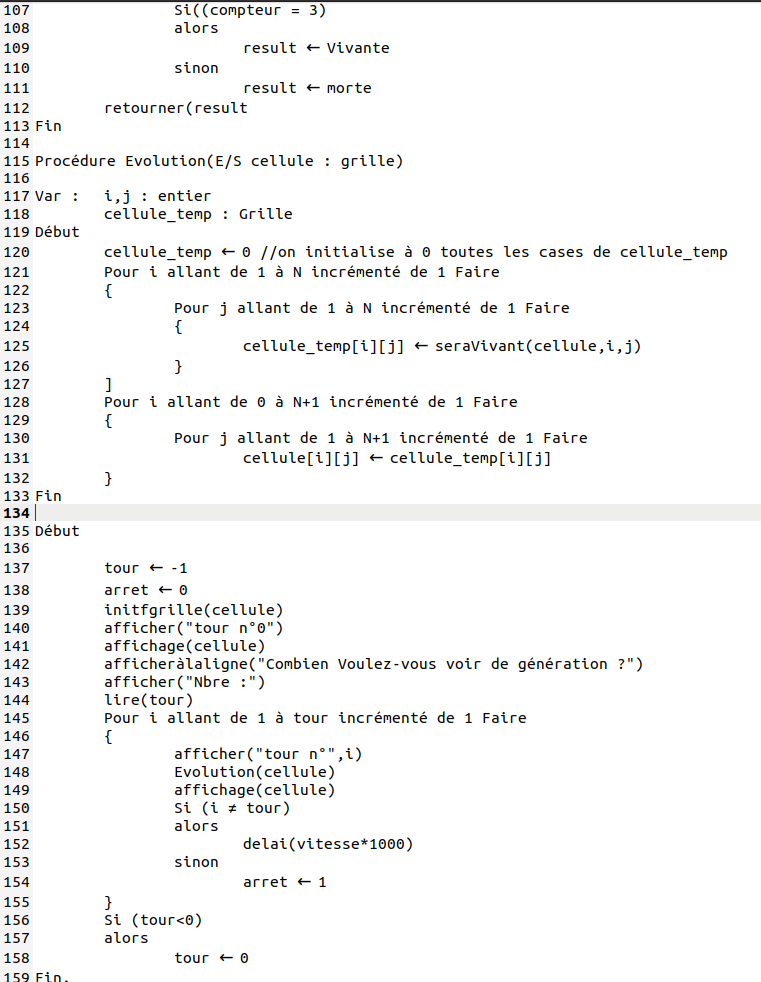
\includegraphics[width=1\textwidth]{./Images/Pseudo_code_3'}\\
	
\end{center}
	
		
\chapter*{Conclusion}

\addcontentsline{toc}{chapter}{Conclusion}

Tout d'abord ce projet a été enrichissant d'un point de vue programmation. En effet l'implémentation de ce programme relativement complexe nous a permis de nous familiariser avec un nouveau langage informatique qu'est le C. N'étant pas familier avec celui-ci, nous avons pu accroître nos compétences dans ce domaine.\\


D'autre part, nous ne connaissions pas le jeu de la vie avant cela. Nous avons donc découvert cette algorithme pourvu de deux règles très simplistes qui, en modélisant, est capable d'engendrer des cas de figure très complexes. Il semble ne pas y avoir de moyen de prédire l'évolution d'un système tiré aléatoirement\\

Cependant, la gestion de la taille du tableau contenant les cellules doit être en théorie infinie. Nous avons dû nous résoudre à travailler avec des dimensions finies à cause du stockage mémoire. Ainsi lorsqu'une structure touche un bord, son comportement ne peut plus être anticipé par le programme.\\

Enfin il a été très enrichissant de pouvoir comparer et compléter deux points de vue différents à l'origine pour arriver à la réalisation finale. Effectivement nous n'avions pas la même façon d'aborder le sujet lorsqu'il a fallu analyser le problème, mais la complémentarité de nos points de vue nous a permis d'arriver à analyser de façon complète le problème.\\

Ce projet nous a permis également à partir d'un problème mathématique, d'en faire un algorithme, pour enfin découvrir tout le potentiel une fois associé à l'implémentation informatique. Cet outil qu'est l'ordinateur se révèle indispensable ici dans la compréhension et l'utilisation d'un objet mathématique à l'origine.\\

La recherche d'animation engendrée par cet algorithme est sans fin, on pourrait s'amuser à en chercher à l'infini.

\chapter*{Annexes}
\addcontentsline{toc}{chapter}{Annexes}

\begin{figure}[H]
	\center
	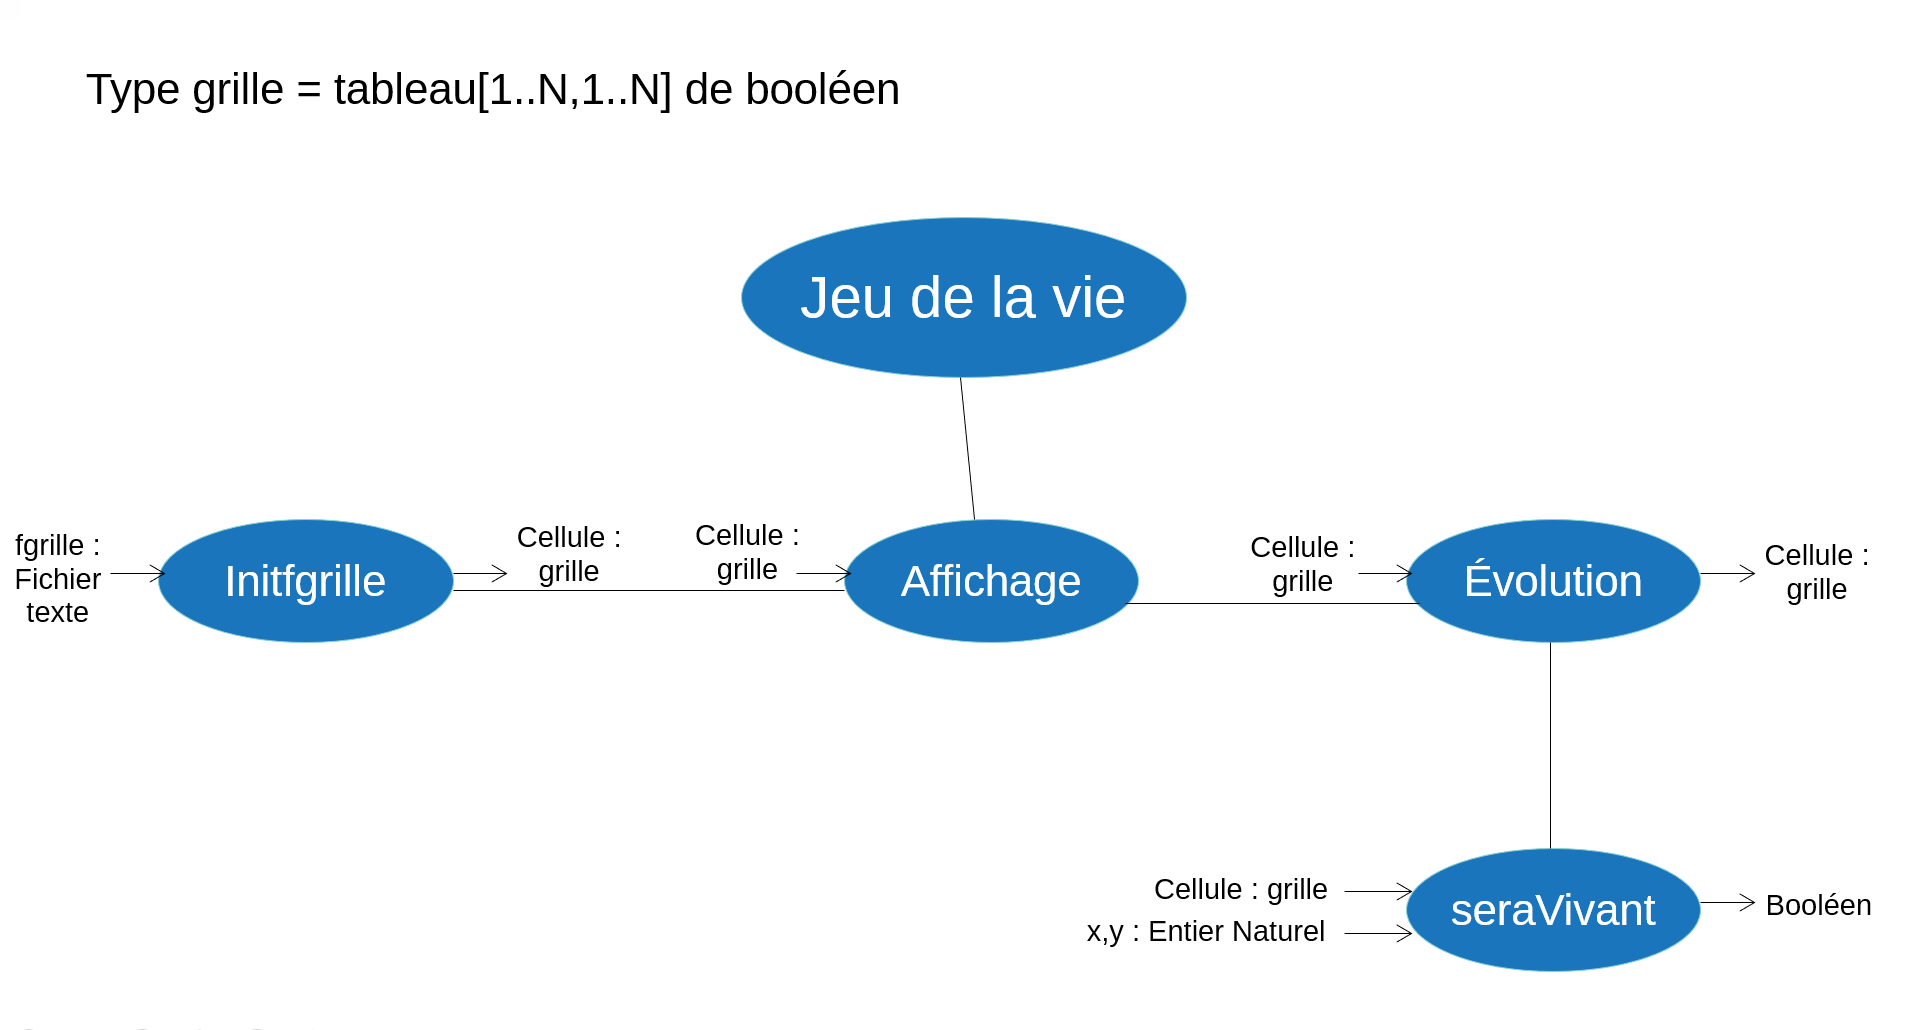
\includegraphics[width=0.9\textwidth]{./Images/Analyse_descendante}
	\caption{Type(s) et Analyse descendante}
\end{figure}\vspace{0.1cm}

\end{document}
